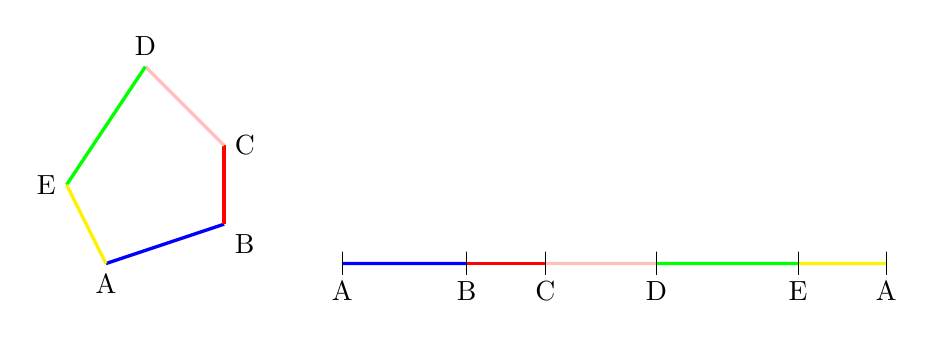
\begin{tikzpicture} % pentagone avec côtés en couleur
\draw [very thick,color=blue] (0,0) node[color=black,below]{A} -- (1.5,0.5) (3,0)--(4.58,0);
\draw [very thick,color=red] (1.5,0.5) node[color=black,below right]{B} -- (1.5,1.5) (4.58,0)--(5.58,0);
\draw [very thick,color=pink] (1.5,1.5) node[color=black,right]{C} -- (0.5,2.5) (5.58,0)--(6.99,0);
\draw [very thick,color=green] (0.5,2.5) node [color=black,above]{D} -- (-0.5,1) (6.99,0)--(8.79,0);
\draw [very thick,color=yellow] (-0.5,1) node[color=black,left]{E} -- (0,0) (8.79,0)--(9.91,0);

\foreach \x / \y in {3/A,4.58/B,5.58/C,6.99/D,8.79/E,9.91/A}
    {\draw (\x,0) node[below=3pt]{\y} --+(0,0.15)--+(0,-0.15);}


\end{tikzpicture} 